\documentclass[1p]{elsarticle_modified}
%\bibliographystyle{elsarticle-num}

%\usepackage[colorlinks]{hyperref}
%\usepackage{abbrmath_seonhwa} %\Abb, \Ascr, \Acal ,\Abf, \Afrak
\usepackage{amsfonts}
\usepackage{amssymb}
\usepackage{amsmath}
\usepackage{amsthm}
\usepackage{scalefnt}
\usepackage{amsbsy}
\usepackage{kotex}
\usepackage{caption}
\usepackage{subfig}
\usepackage{color}
\usepackage{graphicx}
\usepackage{xcolor} %% white, black, red, green, blue, cyan, magenta, yellow
\usepackage{float}
\usepackage{setspace}
\usepackage{hyperref}

\usepackage{tikz}
\usetikzlibrary{arrows}

\usepackage{multirow}
\usepackage{array} % fixed length table
\usepackage{hhline}

%%%%%%%%%%%%%%%%%%%%%
\makeatletter
\renewcommand*\env@matrix[1][\arraystretch]{%
	\edef\arraystretch{#1}%
	\hskip -\arraycolsep
	\let\@ifnextchar\new@ifnextchar
	\array{*\c@MaxMatrixCols c}}
\makeatother %https://tex.stackexchange.com/questions/14071/how-can-i-increase-the-line-spacing-in-a-matrix
%%%%%%%%%%%%%%%

\usepackage[normalem]{ulem}

\newcommand{\msout}[1]{\ifmmode\text{\sout{\ensuremath{#1}}}\else\sout{#1}\fi}
%SOURCE: \msout is \stkout macro in https://tex.stackexchange.com/questions/20609/strikeout-in-math-mode

\newcommand{\cancel}[1]{
	\ifmmode
	{\color{red}\msout{#1}}
	\else
	{\color{red}\sout{#1}}
	\fi
}

\newcommand{\add}[1]{
	{\color{blue}\uwave{#1}}
}

\newcommand{\replace}[2]{
	\ifmmode
	{\color{red}\msout{#1}}{\color{blue}\uwave{#2}}
	\else
	{\color{red}\sout{#1}}{\color{blue}\uwave{#2}}
	\fi
}

\newcommand{\Sol}{\mathcal{S}} %segment
\newcommand{\D}{D} %diagram
\newcommand{\A}{\mathcal{A}} %arc


%%%%%%%%%%%%%%%%%%%%%%%%%%%%%5 test

\def\sl{\operatorname{\textup{SL}}(2,\Cbb)}
\def\psl{\operatorname{\textup{PSL}}(2,\Cbb)}
\def\quan{\mkern 1mu \triangleright \mkern 1mu}

\theoremstyle{definition}
\newtheorem{thm}{Theorem}[section]
\newtheorem{prop}[thm]{Proposition}
\newtheorem{lem}[thm]{Lemma}
\newtheorem{ques}[thm]{Question}
\newtheorem{cor}[thm]{Corollary}
\newtheorem{defn}[thm]{Definition}
\newtheorem{exam}[thm]{Example}
\newtheorem{rmk}[thm]{Remark}
\newtheorem{alg}[thm]{Algorithm}

\newcommand{\I}{\sqrt{-1}}
\begin{document}

%\begin{frontmatter}
%
%\title{Boundary parabolic representations of knots up to 8 crossings}
%
%%% Group authors per affiliation:
%\author{Yunhi Cho} 
%\address{Department of Mathematics, University of Seoul, Seoul, Korea}
%\ead{yhcho@uos.ac.kr}
%
%
%\author{Seonhwa Kim} %\fnref{s_kim}}
%\address{Center for Geometry and Physics, Institute for Basic Science, Pohang, 37673, Korea}
%\ead{ryeona17@ibs.re.kr}
%
%\author{Hyuk Kim}
%\address{Department of Mathematical Sciences, Seoul National University, Seoul 08826, Korea}
%\ead{hyukkim@snu.ac.kr}
%
%\author{Seokbeom Yoon}
%\address{Department of Mathematical Sciences, Seoul National University, Seoul, 08826,  Korea}
%\ead{sbyoon15@snu.ac.kr}
%
%\begin{abstract}
%We find all boundary parabolic representation of knots up to 8 crossings.
%
%\end{abstract}
%\begin{keyword}
%    \MSC[2010] 57M25 
%\end{keyword}
%
%\end{frontmatter}

%\linenumbers
%\tableofcontents
%
\newcommand\colored[1]{\textcolor{white}{\rule[-0.35ex]{0.8em}{1.4ex}}\kern-0.8em\color{red} #1}%
%\newcommand\colored[1]{\textcolor{white}{ #1}\kern-2.17ex	\textcolor{white}{ #1}\kern-1.81ex	\textcolor{white}{ #1}\kern-2.15ex\color{red}#1	}

{\Large $\underline{12n_{0886}~(K12n_{0886})}$}

\setlength{\tabcolsep}{10pt}
\renewcommand{\arraystretch}{1.6}
\vspace{1cm}\begin{tabular}{m{100pt}>{\centering\arraybackslash}m{274pt}}
\multirow{5}{120pt}{
	\centering
	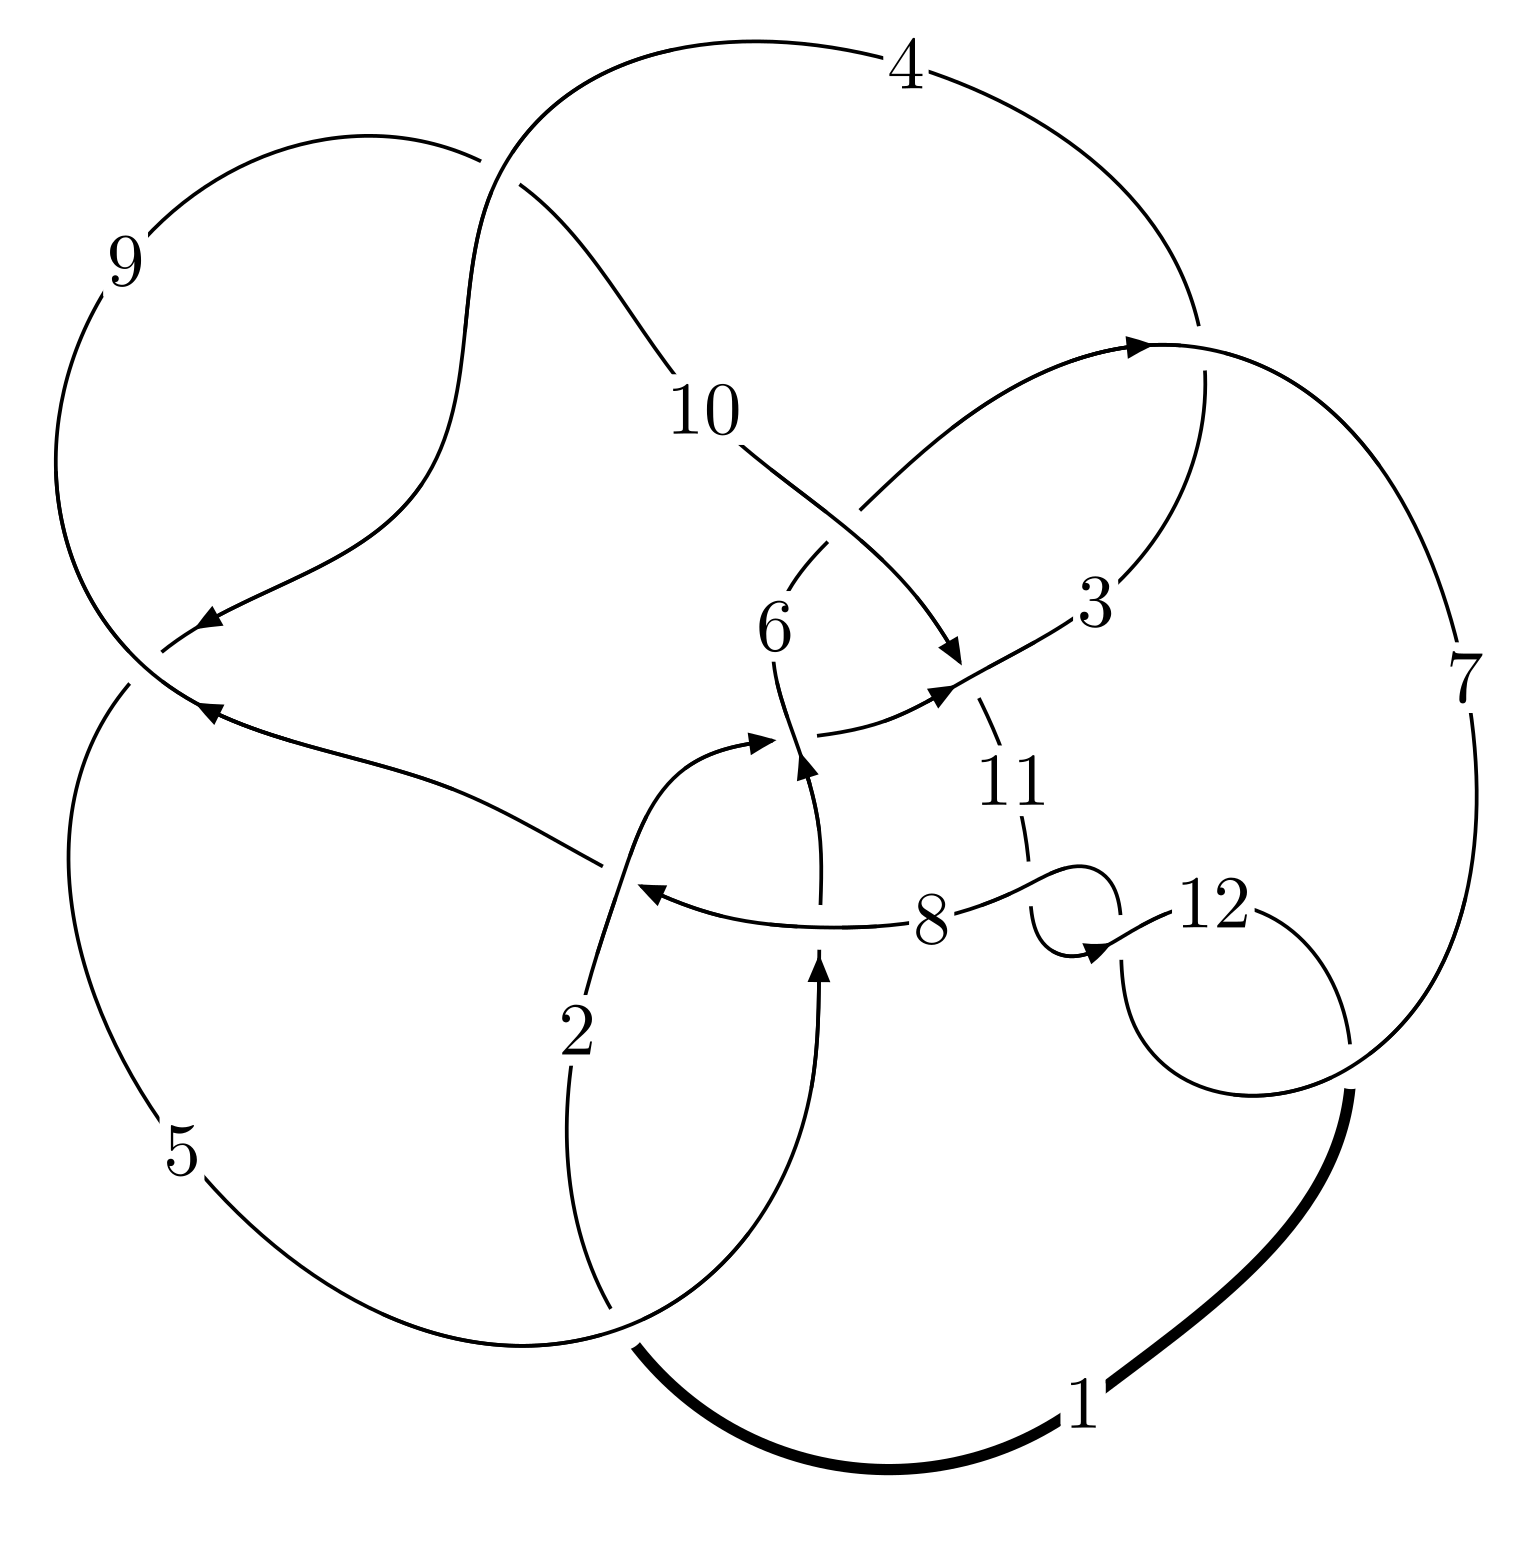
\includegraphics[width=112pt]{../../../GIT/diagram.site/Diagrams/png/2975_12n_0886.png}\\
\ \ \ A knot diagram\footnotemark}&
\allowdisplaybreaks
\textbf{Linearized knot diagam} \\
\cline{2-2}
 &
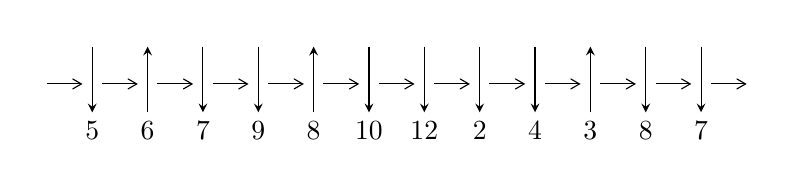
\begin{tikzpicture}[x=20pt, y=17pt]
	% nodes
	\node (C0) at (0, 0) {};
	\node (C1) at (1, 0) {};
	\node (C1U) at (1, +1) {};
	\node (C1D) at (1, -1) {5};

	\node (C2) at (2, 0) {};
	\node (C2U) at (2, +1) {};
	\node (C2D) at (2, -1) {6};

	\node (C3) at (3, 0) {};
	\node (C3U) at (3, +1) {};
	\node (C3D) at (3, -1) {7};

	\node (C4) at (4, 0) {};
	\node (C4U) at (4, +1) {};
	\node (C4D) at (4, -1) {9};

	\node (C5) at (5, 0) {};
	\node (C5U) at (5, +1) {};
	\node (C5D) at (5, -1) {8};

	\node (C6) at (6, 0) {};
	\node (C6U) at (6, +1) {};
	\node (C6D) at (6, -1) {10};

	\node (C7) at (7, 0) {};
	\node (C7U) at (7, +1) {};
	\node (C7D) at (7, -1) {12};

	\node (C8) at (8, 0) {};
	\node (C8U) at (8, +1) {};
	\node (C8D) at (8, -1) {2};

	\node (C9) at (9, 0) {};
	\node (C9U) at (9, +1) {};
	\node (C9D) at (9, -1) {4};

	\node (C10) at (10, 0) {};
	\node (C10U) at (10, +1) {};
	\node (C10D) at (10, -1) {3};

	\node (C11) at (11, 0) {};
	\node (C11U) at (11, +1) {};
	\node (C11D) at (11, -1) {8};

	\node (C12) at (12, 0) {};
	\node (C12U) at (12, +1) {};
	\node (C12D) at (12, -1) {7};
	\node (C13) at (13, 0) {};

	% arrows
	\draw[->,>={angle 60}]
	(C0) edge (C1) (C1) edge (C2) (C2) edge (C3) (C3) edge (C4) (C4) edge (C5) (C5) edge (C6) (C6) edge (C7) (C7) edge (C8) (C8) edge (C9) (C9) edge (C10) (C10) edge (C11) (C11) edge (C12) (C12) edge (C13) ;	\draw[->,>=stealth]
	(C1U) edge (C1D) (C2D) edge (C2U) (C3U) edge (C3D) (C4U) edge (C4D) (C5D) edge (C5U) (C6U) edge (C6D) (C7U) edge (C7D) (C8U) edge (C8D) (C9U) edge (C9D) (C10D) edge (C10U) (C11U) edge (C11D) (C12U) edge (C12D) ;
	\end{tikzpicture} \\
\hhline{~~} \\& 
\textbf{Solving Sequence} \\ \cline{2-2} 
 &
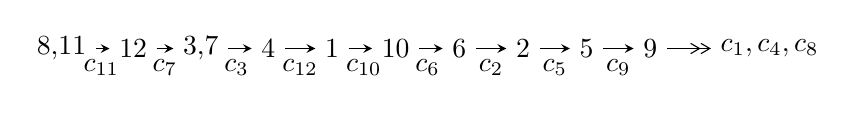
\begin{tikzpicture}[x=23pt, y=7pt]
	% node
	\node (A0) at (-1/8, 0) {8,11};
	\node (A1) at (1, 0) {12};
	\node (A2) at (33/16, 0) {3,7};
	\node (A3) at (25/8, 0) {4};
	\node (A4) at (33/8, 0) {1};
	\node (A5) at (41/8, 0) {10};
	\node (A6) at (49/8, 0) {6};
	\node (A7) at (57/8, 0) {2};
	\node (A8) at (65/8, 0) {5};
	\node (A9) at (73/8, 0) {9};
	\node (C1) at (1/2, -1) {$c_{11}$};
	\node (C2) at (3/2, -1) {$c_{7}$};
	\node (C3) at (21/8, -1) {$c_{3}$};
	\node (C4) at (29/8, -1) {$c_{12}$};
	\node (C5) at (37/8, -1) {$c_{10}$};
	\node (C6) at (45/8, -1) {$c_{6}$};
	\node (C7) at (53/8, -1) {$c_{2}$};
	\node (C8) at (61/8, -1) {$c_{5}$};
	\node (C9) at (69/8, -1) {$c_{9}$};
	\node (A10) at (11, 0) {$c_{1},c_{4},c_{8}$};

	% edge
	\draw[->,>=stealth]	
	(A0) edge (A1) (A1) edge (A2) (A2) edge (A3) (A3) edge (A4) (A4) edge (A5) (A5) edge (A6) (A6) edge (A7) (A7) edge (A8) (A8) edge (A9) ;
	\draw[->>,>={angle 60}]	
	(A9) edge (A10);
\end{tikzpicture} \\ 

\end{tabular} \\

\footnotetext{
The image of knot diagram is generated by the software ``\textbf{Draw programme}" developed by Andrew Bartholomew(\url{http://www.layer8.co.uk/maths/draw/index.htm\#Running-draw}), where we modified some parts for our purpose(\url{https://github.com/CATsTAILs/LinksPainter}).
}\phantom \\ \newline 
\centering \textbf{Ideals for irreducible components\footnotemark of $X_{\text{par}}$} 
 
\begin{align*}
I^u_{1}&=\langle 
2.28947\times10^{47} u^{38}+4.04764\times10^{47} u^{37}+\cdots+2.48782\times10^{48} b-5.46868\times10^{48},\\
\phantom{I^u_{1}}&\phantom{= \langle  }4.40280\times10^{48} u^{38}+1.28334\times10^{49} u^{37}+\cdots+3.48294\times10^{49} a+1.28461\times10^{49},\;u^{39}+3 u^{38}+\cdots+97 u+28\rangle \\
I^u_{2}&=\langle 
-3.16826\times10^{23} a u^{35}+4.21892\times10^{23} u^{35}+\cdots+6.95896\times10^{24} a+5.71717\times10^{24},\\
\phantom{I^u_{2}}&\phantom{= \langle  }5.19604\times10^{24} a u^{35}-8.48983\times10^{24} u^{35}+\cdots+6.84613\times10^{24} a+1.19689\times10^{26},\\
\phantom{I^u_{2}}&\phantom{= \langle  }u^{36}-2 u^{35}+\cdots-48 u+19\rangle \\
I^u_{3}&=\langle 
-22 u^{12} a+31 u^{12}+\cdots+12 a+9,\;6 u^{12} a+4 u^{12}+\cdots-6 a+38,\\
\phantom{I^u_{3}}&\phantom{= \langle  }u^{13}-2 u^{12}+8 u^{11}-12 u^{10}+25 u^9-27 u^8+40 u^7-31 u^6+36 u^5-18 u^4+17 u^3-2 u^2+3 u+1\rangle \\
I^u_{4}&=\langle 
- u^5-2 u^4-3 u^3-3 u^2+b-2 u,\;- u^4-2 u^3-4 u^2+a-3 u-3,\;u^6+2 u^5+4 u^4+4 u^3+4 u^2+u+1\rangle \\
\\
\end{align*}
\raggedright * 4 irreducible components of $\dim_{\mathbb{C}}=0$, with total 143 representations.\\
\footnotetext{All coefficients of polynomials are rational numbers. But the coefficients are sometimes approximated in decimal forms when there is not enough margin.}
\newpage
\renewcommand{\arraystretch}{1}
\centering \section*{I. $I^u_{1}= \langle 2.29\times10^{47} u^{38}+4.05\times10^{47} u^{37}+\cdots+2.49\times10^{48} b-5.47\times10^{48},\;4.40\times10^{48} u^{38}+1.28\times10^{49} u^{37}+\cdots+3.48\times10^{49} a+1.28\times10^{49},\;u^{39}+3 u^{38}+\cdots+97 u+28 \rangle$}
\flushleft \textbf{(i) Arc colorings}\\
\begin{tabular}{m{7pt} m{180pt} m{7pt} m{180pt} }
\flushright $a_{8}=$&$\begin{pmatrix}0\\u\end{pmatrix}$ \\
\flushright $a_{11}=$&$\begin{pmatrix}1\\0\end{pmatrix}$ \\
\flushright $a_{12}=$&$\begin{pmatrix}1\\u^2\end{pmatrix}$ \\
\flushright $a_{3}=$&$\begin{pmatrix}-0.126410 u^{38}-0.368465 u^{37}+\cdots-11.5215 u-0.368828\\-0.0920273 u^{38}-0.162698 u^{37}+\cdots+2.33867 u+2.19819\end{pmatrix}$ \\
\flushright $a_{7}=$&$\begin{pmatrix}u\\u^3+u\end{pmatrix}$ \\
\flushright $a_{4}=$&$\begin{pmatrix}-0.126011 u^{38}-0.302424 u^{37}+\cdots-3.73851 u+1.95256\\-0.104356 u^{38}-0.190877 u^{37}+\cdots+3.82088 u+2.70401\end{pmatrix}$ \\
\flushright $a_{1}=$&$\begin{pmatrix}u^2+1\\u^4+2 u^2\end{pmatrix}$ \\
\flushright $a_{10}=$&$\begin{pmatrix}-0.194866 u^{38}-0.476802 u^{37}+\cdots-9.00949 u-1.31112\\0.0407147 u^{38}-0.0606632 u^{37}+\cdots-11.8899 u-6.06492\end{pmatrix}$ \\
\flushright $a_{6}=$&$\begin{pmatrix}-0.0785067 u^{38}-0.327547 u^{37}+\cdots-14.6147 u-5.27648\\0.0107661 u^{38}+0.0759285 u^{37}+\cdots+11.8930 u+3.53949\end{pmatrix}$ \\
\flushright $a_{2}=$&$\begin{pmatrix}-0.113492 u^{38}-0.284012 u^{37}+\cdots-2.11951 u+1.73553\\0.195599 u^{38}+0.486101 u^{37}+\cdots+11.1853 u+0.740865\end{pmatrix}$ \\
\flushright $a_{5}=$&$\begin{pmatrix}-0.0785067 u^{38}-0.327547 u^{37}+\cdots-14.6147 u-5.27648\\0.124150 u^{38}+0.411280 u^{37}+\cdots+23.0178 u+6.11626\end{pmatrix}$ \\
\flushright $a_{9}=$&$\begin{pmatrix}-0.0241106 u^{38}+0.0681245 u^{37}+\cdots+15.3829 u+6.23920\\0.225516 u^{38}+0.613536 u^{37}+\cdots+12.0478 u+0.558854\end{pmatrix}$\\&\end{tabular}
\flushleft \textbf{(ii) Obstruction class $= -1$}\\~\\
\flushleft \textbf{(iii) Cusp Shapes $= -0.711169 u^{38}-3.04251 u^{37}+\cdots-97.9978 u-38.0725$}\\~\\
\newpage\renewcommand{\arraystretch}{1}
\flushleft \textbf{(iv) u-Polynomials at the component}\newline \\
\begin{tabular}{m{50pt}|m{274pt}}
Crossings & \hspace{64pt}u-Polynomials at each crossing \\
\hline $$\begin{aligned}c_{1},c_{3}\end{aligned}$$&$\begin{aligned}
&u^{39}- u^{38}+\cdots-288 u+24
\end{aligned}$\\
\hline $$\begin{aligned}c_{2}\end{aligned}$$&$\begin{aligned}
&u^{39}-6 u^{38}+\cdots+577 u+284
\end{aligned}$\\
\hline $$\begin{aligned}c_{4},c_{9}\end{aligned}$$&$\begin{aligned}
&3(3 u^{39}-9 u^{38}+\cdots+384 u+128)
\end{aligned}$\\
\hline $$\begin{aligned}c_{5},c_{10}\end{aligned}$$&$\begin{aligned}
&3(3 u^{39}-15 u^{38}+\cdots+24 u+17)
\end{aligned}$\\
\hline $$\begin{aligned}c_{6},c_{8}\end{aligned}$$&$\begin{aligned}
&u^{39}+4 u^{37}+\cdots-21 u+3
\end{aligned}$\\
\hline $$\begin{aligned}c_{7},c_{11},c_{12}\end{aligned}$$&$\begin{aligned}
&u^{39}+3 u^{38}+\cdots+97 u+28
\end{aligned}$\\
\hline
\end{tabular}\\~\\
\newpage\renewcommand{\arraystretch}{1}
\flushleft \textbf{(v) Riley Polynomials at the component}\newline \\
\begin{tabular}{m{50pt}|m{274pt}}
Crossings & \hspace{64pt}Riley Polynomials at each crossing \\
\hline $$\begin{aligned}c_{1},c_{3}\end{aligned}$$&$\begin{aligned}
&y^{39}-13 y^{38}+\cdots+9024 y-576
\end{aligned}$\\
\hline $$\begin{aligned}c_{2}\end{aligned}$$&$\begin{aligned}
&y^{39}+10 y^{38}+\cdots+1402473 y-80656
\end{aligned}$\\
\hline $$\begin{aligned}c_{4},c_{9}\end{aligned}$$&$\begin{aligned}
&9(9 y^{39}+165 y^{38}+\cdots+188416 y-16384)
\end{aligned}$\\
\hline $$\begin{aligned}c_{5},c_{10}\end{aligned}$$&$\begin{aligned}
&9(9 y^{39}+147 y^{38}+\cdots-7176 y-289)
\end{aligned}$\\
\hline $$\begin{aligned}c_{6},c_{8}\end{aligned}$$&$\begin{aligned}
&y^{39}+8 y^{38}+\cdots+69 y-9
\end{aligned}$\\
\hline $$\begin{aligned}c_{7},c_{11},c_{12}\end{aligned}$$&$\begin{aligned}
&y^{39}+19 y^{38}+\cdots+3249 y-784
\end{aligned}$\\
\hline
\end{tabular}\\~\\
\newpage\flushleft \textbf{(vi) Complex Volumes and Cusp Shapes}
$$\begin{array}{c|c|c}  
\text{Solutions to }I^u_{1}& \I (\text{vol} + \sqrt{-1}CS) & \text{Cusp shape}\\
 \hline 
\begin{aligned}
u &= -0.916514 + 0.441237 I \\
a &= \phantom{-}0.247881 - 0.833626 I \\
b &= \phantom{-}0.207591 - 1.107760 I\end{aligned}
 & -2.80770 + 1.03926 I & -7.88545 - 0.44169 I \\ \hline\begin{aligned}
u &= -0.916514 - 0.441237 I \\
a &= \phantom{-}0.247881 + 0.833626 I \\
b &= \phantom{-}0.207591 + 1.107760 I\end{aligned}
 & -2.80770 - 1.03926 I & -7.88545 + 0.44169 I \\ \hline\begin{aligned}
u &= -0.135804 + 0.949926 I \\
a &= -0.160880 - 1.247510 I \\
b &= \phantom{-}0.883058 + 0.239291 I\end{aligned}
 & \phantom{-}4.06880 + 6.12048 I & \phantom{-}0.19446 - 7.21984 I \\ \hline\begin{aligned}
u &= -0.135804 - 0.949926 I \\
a &= -0.160880 + 1.247510 I \\
b &= \phantom{-}0.883058 - 0.239291 I\end{aligned}
 & \phantom{-}4.06880 - 6.12048 I & \phantom{-}0.19446 + 7.21984 I \\ \hline\begin{aligned}
u &= -0.328914 + 0.888085 I \\
a &= -0.161668 - 1.131530 I \\
b &= -1.237060 - 0.045140 I\end{aligned}
 & \phantom{-}1.48517 + 2.10751 I & -1.96614 - 8.73804 I \\ \hline\begin{aligned}
u &= -0.328914 - 0.888085 I \\
a &= -0.161668 + 1.131530 I \\
b &= -1.237060 + 0.045140 I\end{aligned}
 & \phantom{-}1.48517 - 2.10751 I & -1.96614 + 8.73804 I \\ \hline\begin{aligned}
u &= -0.483608 + 0.797162 I \\
a &= \phantom{-}0.47424 - 2.55899 I \\
b &= -1.82147 - 1.40610 I\end{aligned}
 & \phantom{-}1.57165 + 2.07582 I & \phantom{-}13.4964 + 12.8859 I \\ \hline\begin{aligned}
u &= -0.483608 - 0.797162 I \\
a &= \phantom{-}0.47424 + 2.55899 I \\
b &= -1.82147 + 1.40610 I\end{aligned}
 & \phantom{-}1.57165 - 2.07582 I & \phantom{-}13.4964 - 12.8859 I \\ \hline\begin{aligned}
u &= \phantom{-}0.923741 + 0.613959 I \\
a &= -0.890068 - 0.882613 I \\
b &= -0.80569 - 1.43771 I\end{aligned}
 & -3.92945 + 6.07851 I & -7.89096 - 4.82336 I \\ \hline\begin{aligned}
u &= \phantom{-}0.923741 - 0.613959 I \\
a &= -0.890068 + 0.882613 I \\
b &= -0.80569 + 1.43771 I\end{aligned}
 & -3.92945 - 6.07851 I & -7.89096 + 4.82336 I\\
 \hline 
 \end{array}$$\newpage$$\begin{array}{c|c|c}  
\text{Solutions to }I^u_{1}& \I (\text{vol} + \sqrt{-1}CS) & \text{Cusp shape}\\
 \hline 
\begin{aligned}
u &= -0.752187 + 0.832147 I \\
a &= \phantom{-}1.13539 - 0.96953 I \\
b &= -0.190145 - 0.615515 I\end{aligned}
 & -0.10015 - 2.41578 I & -8.63287 + 3.83598 I \\ \hline\begin{aligned}
u &= -0.752187 - 0.832147 I \\
a &= \phantom{-}1.13539 + 0.96953 I \\
b &= -0.190145 + 0.615515 I\end{aligned}
 & -0.10015 + 2.41578 I & -8.63287 - 3.83598 I \\ \hline\begin{aligned}
u &= -0.711955 + 0.900911 I \\
a &= -0.089276 - 1.410670 I \\
b &= -0.089221 - 0.908822 I\end{aligned}
 & \phantom{-}0.11878 + 7.97565 I & -8.57990 - 9.49272 I \\ \hline\begin{aligned}
u &= -0.711955 - 0.900911 I \\
a &= -0.089276 + 1.410670 I \\
b &= -0.089221 + 0.908822 I\end{aligned}
 & \phantom{-}0.11878 - 7.97565 I & -8.57990 + 9.49272 I \\ \hline\begin{aligned}
u &= \phantom{-}0.800506 + 0.823754 I \\
a &= \phantom{-}0.212411 + 1.237080 I \\
b &= -0.125997 + 1.041490 I\end{aligned}
 & -4.29233 - 4.38952 I & -12.7464 + 8.5386 I \\ \hline\begin{aligned}
u &= \phantom{-}0.800506 - 0.823754 I \\
a &= \phantom{-}0.212411 - 1.237080 I \\
b &= -0.125997 - 1.041490 I\end{aligned}
 & -4.29233 + 4.38952 I & -12.7464 - 8.5386 I \\ \hline\begin{aligned}
u &= \phantom{-}0.713165 + 0.944690 I \\
a &= \phantom{-}0.925475 + 0.938504 I \\
b &= -0.208623 + 0.798757 I\end{aligned}
 & -3.87382 - 1.34228 I & -11.55865 - 0.85858 I \\ \hline\begin{aligned}
u &= \phantom{-}0.713165 - 0.944690 I \\
a &= \phantom{-}0.925475 - 0.938504 I \\
b &= -0.208623 - 0.798757 I\end{aligned}
 & -3.87382 + 1.34228 I & -11.55865 + 0.85858 I \\ \hline\begin{aligned}
u &= -0.177652 + 0.777872 I \\
a &= \phantom{-}1.70436 + 0.68558 I \\
b &= -0.822667 + 0.609797 I\end{aligned}
 & \phantom{-}3.36049 - 4.70428 I & \phantom{-}0.07633 + 7.03063 I \\ \hline\begin{aligned}
u &= -0.177652 - 0.777872 I \\
a &= \phantom{-}1.70436 - 0.68558 I \\
b &= -0.822667 - 0.609797 I\end{aligned}
 & \phantom{-}3.36049 + 4.70428 I & \phantom{-}0.07633 - 7.03063 I\\
 \hline 
 \end{array}$$\newpage$$\begin{array}{c|c|c}  
\text{Solutions to }I^u_{1}& \I (\text{vol} + \sqrt{-1}CS) & \text{Cusp shape}\\
 \hline 
\begin{aligned}
u &= -1.146750 + 0.440730 I \\
a &= -0.565258 + 0.986647 I \\
b &= -0.89775 + 1.37606 I\end{aligned}
 & \phantom{-}0.05936 - 12.21210 I & -4.60084 + 6.75366 I \\ \hline\begin{aligned}
u &= -1.146750 - 0.440730 I \\
a &= -0.565258 - 0.986647 I \\
b &= -0.89775 - 1.37606 I\end{aligned}
 & \phantom{-}0.05936 + 12.21210 I & -4.60084 - 6.75366 I \\ \hline\begin{aligned}
u &= \phantom{-}0.735638 + 1.075410 I \\
a &= -0.76266 - 1.50039 I \\
b &= \phantom{-}1.16251 - 1.43644 I\end{aligned}
 & -2.50894 - 12.16870 I & -6.00000 + 9.67889 I \\ \hline\begin{aligned}
u &= \phantom{-}0.735638 - 1.075410 I \\
a &= -0.76266 + 1.50039 I \\
b &= \phantom{-}1.16251 + 1.43644 I\end{aligned}
 & -2.50894 + 12.16870 I & -6.00000 - 9.67889 I \\ \hline\begin{aligned}
u &= -0.617583 + 1.166490 I \\
a &= \phantom{-}0.802084 - 0.731744 I \\
b &= -0.520402 - 0.991081 I\end{aligned}
 & -0.54733 + 4.60938 I & -6.00000 - 4.32150 I \\ \hline\begin{aligned}
u &= -0.617583 - 1.166490 I \\
a &= \phantom{-}0.802084 + 0.731744 I \\
b &= -0.520402 + 0.991081 I\end{aligned}
 & -0.54733 - 4.60938 I & -6.00000 + 4.32150 I \\ \hline\begin{aligned}
u &= \phantom{-}0.177150 + 1.362390 I \\
a &= -0.738434 + 0.517093 I \\
b &= \phantom{-}0.110360 - 0.283380 I\end{aligned}
 & \phantom{-}8.80818 - 3.56269 I & \phantom{-0.000000 } 0 \\ \hline\begin{aligned}
u &= \phantom{-}0.177150 - 1.362390 I \\
a &= -0.738434 - 0.517093 I \\
b &= \phantom{-}0.110360 + 0.283380 I\end{aligned}
 & \phantom{-}8.80818 + 3.56269 I & \phantom{-0.000000 } 0 \\ \hline\begin{aligned}
u &= -0.09539 + 1.41424 I \\
a &= -0.264813 - 0.436944 I \\
b &= \phantom{-}0.341868 + 0.804996 I\end{aligned}
 & \phantom{-}3.95195 + 4.10222 I & -13.18136 + 0. I\phantom{ +0.000000I} \\ \hline\begin{aligned}
u &= -0.09539 - 1.41424 I \\
a &= -0.264813 + 0.436944 I \\
b &= \phantom{-}0.341868 - 0.804996 I\end{aligned}
 & \phantom{-}3.95195 - 4.10222 I & -13.18136 + 0. I\phantom{ +0.000000I}\\
 \hline 
 \end{array}$$\newpage$$\begin{array}{c|c|c}  
\text{Solutions to }I^u_{1}& \I (\text{vol} + \sqrt{-1}CS) & \text{Cusp shape}\\
 \hline 
\begin{aligned}
u &= -0.74692 + 1.23578 I \\
a &= -0.84084 + 1.29226 I \\
b &= \phantom{-}1.11567 + 1.33283 I\end{aligned}
 & \phantom{-}2.5485 + 18.9404 I & \phantom{-0.000000 } 0 \\ \hline\begin{aligned}
u &= -0.74692 - 1.23578 I \\
a &= -0.84084 - 1.29226 I \\
b &= \phantom{-}1.11567 - 1.33283 I\end{aligned}
 & \phantom{-}2.5485 - 18.9404 I & \phantom{-0.000000 } 0 \\ \hline\begin{aligned}
u &= \phantom{-}1.11970 + 0.93154 I \\
a &= \phantom{-}0.408674 + 0.839692 I \\
b &= -0.125452 + 1.366430 I\end{aligned}
 & -3.17217 - 3.88150 I & \phantom{-0.000000 } 0 \\ \hline\begin{aligned}
u &= \phantom{-}1.11970 - 0.93154 I \\
a &= \phantom{-}0.408674 - 0.839692 I \\
b &= -0.125452 - 1.366430 I\end{aligned}
 & -3.17217 + 3.88150 I & \phantom{-0.000000 } 0 \\ \hline\begin{aligned}
u &= \phantom{-}0.442258 + 0.222040 I \\
a &= \phantom{-}1.168930 - 0.401308 I \\
b &= -0.226973 + 0.541420 I\end{aligned}
 & \phantom{-}3.75967 - 1.17014 I & -3.19480 + 5.79771 I \\ \hline\begin{aligned}
u &= \phantom{-}0.442258 - 0.222040 I \\
a &= \phantom{-}1.168930 + 0.401308 I \\
b &= -0.226973 - 0.541420 I\end{aligned}
 & \phantom{-}3.75967 + 1.17014 I & -3.19480 - 5.79771 I \\ \hline\begin{aligned}
u &= -0.13386 + 1.60465 I \\
a &= -0.048505 + 0.218993 I \\
b &= \phantom{-}0.580718 - 1.138840 I\end{aligned}
 & \phantom{-}7.49768 - 7.41295 I & \phantom{-0.000000 } 0 \\ \hline\begin{aligned}
u &= -0.13386 - 1.60465 I \\
a &= -0.048505 - 0.218993 I \\
b &= \phantom{-}0.580718 + 1.138840 I\end{aligned}
 & \phantom{-}7.49768 + 7.41295 I & \phantom{-0.000000 } 0 \\ \hline\begin{aligned}
u &= -0.330056\phantom{ +0.000000I} \\
a &= \phantom{-}1.27880\phantom{ +0.000000I} \\
b &= \phantom{-}0.339349\phantom{ +0.000000I}\end{aligned}
 & -0.743035\phantom{ +0.000000I} & -13.5950\phantom{ +0.000000I}\\
 \hline 
 \end{array}$$\newpage\newpage\renewcommand{\arraystretch}{1}
\centering \section*{II. $I^u_{2}= \langle -3.17\times10^{23} a u^{35}+4.22\times10^{23} u^{35}+\cdots+6.96\times10^{24} a+5.72\times10^{24},\;5.20\times10^{24} a u^{35}-8.49\times10^{24} u^{35}+\cdots+6.85\times10^{24} a+1.20\times10^{26},\;u^{36}-2 u^{35}+\cdots-48 u+19 \rangle$}
\flushleft \textbf{(i) Arc colorings}\\
\begin{tabular}{m{7pt} m{180pt} m{7pt} m{180pt} }
\flushright $a_{8}=$&$\begin{pmatrix}0\\u\end{pmatrix}$ \\
\flushright $a_{11}=$&$\begin{pmatrix}1\\0\end{pmatrix}$ \\
\flushright $a_{12}=$&$\begin{pmatrix}1\\u^2\end{pmatrix}$ \\
\flushright $a_{3}=$&$\begin{pmatrix}a\\2.06053 a u^{35}-2.74385 u^{35}+\cdots-45.2588 a-37.1826\end{pmatrix}$ \\
\flushright $a_{7}=$&$\begin{pmatrix}u\\u^3+u\end{pmatrix}$ \\
\flushright $a_{4}=$&$\begin{pmatrix}1.48264 a u^{35}-1.81640 u^{35}+\cdots-25.3448 a-27.0290\\2.57849 a u^{35}-3.07539 u^{35}+\cdots-56.3149 a-44.1527\end{pmatrix}$ \\
\flushright $a_{1}=$&$\begin{pmatrix}u^2+1\\u^4+2 u^2\end{pmatrix}$ \\
\flushright $a_{10}=$&$\begin{pmatrix}1.06765 a u^{35}-0.157828 u^{35}+\cdots-25.9276 a+24.1903\\-1.00977 a u^{35}+2.51580 u^{35}+\cdots+30.5478 a-48.9528\end{pmatrix}$ \\
\flushright $a_{6}=$&$\begin{pmatrix}-2.38204 a u^{35}+1.36461 u^{35}+\cdots-49.5905 a+25.0494\\0.374254 u^{35}+0.716994 u^{34}+\cdots-189.282 u+72.9225\end{pmatrix}$ \\
\flushright $a_{2}=$&$\begin{pmatrix}-0.913044 a u^{35}+2.61003 u^{35}+\cdots+28.4338 a-73.4659\\-1.71093 a u^{35}+2.45734 u^{35}+\cdots-0.462668 a-176.281\end{pmatrix}$ \\
\flushright $a_{5}=$&$\begin{pmatrix}-2.38204 a u^{35}+1.36461 u^{35}+\cdots-49.5905 a+25.0494\\1.38657 a u^{35}-1.10162 u^{35}+\cdots+39.1501 a+52.6371\end{pmatrix}$ \\
\flushright $a_{9}=$&$\begin{pmatrix}-0.995475 a u^{35}-0.534403 u^{35}+\cdots-10.4404 a+39.4763\\0.860915 a u^{35}+2.29603 u^{35}+\cdots-34.0245 a-24.9123\end{pmatrix}$\\&\end{tabular}
\flushleft \textbf{(ii) Obstruction class $= -1$}\\~\\
\flushleft \textbf{(iii) Cusp Shapes $= -\frac{93144148804390001398740}{3750225582640850341841} u^{35}+\frac{92757417872856011479263}{3750225582640850341841} u^{34}+\cdots+\frac{3062243866116418648517160}{3750225582640850341841} u-\frac{2323290663795802739504375}{3750225582640850341841}$}\\~\\
\newpage\renewcommand{\arraystretch}{1}
\flushleft \textbf{(iv) u-Polynomials at the component}\newline \\
\begin{tabular}{m{50pt}|m{274pt}}
Crossings & \hspace{64pt}u-Polynomials at each crossing \\
\hline $$\begin{aligned}c_{1},c_{3}\end{aligned}$$&$\begin{aligned}
&u^{72}+u^{71}+\cdots+2338 u+157
\end{aligned}$\\
\hline $$\begin{aligned}c_{2}\end{aligned}$$&$\begin{aligned}
&(u^{36}+3 u^{35}+\cdots-4 u+1)^{2}
\end{aligned}$\\
\hline $$\begin{aligned}c_{4},c_{9}\end{aligned}$$&$\begin{aligned}
&(u^{36}- u^{35}+\cdots-414 u+81)^{2}
\end{aligned}$\\
\hline $$\begin{aligned}c_{5},c_{10}\end{aligned}$$&$\begin{aligned}
&u^{72}-10 u^{70}+\cdots-504 u+281
\end{aligned}$\\
\hline $$\begin{aligned}c_{6},c_{8}\end{aligned}$$&$\begin{aligned}
&u^{72}+u^{71}+\cdots+112 u+263
\end{aligned}$\\
\hline $$\begin{aligned}c_{7},c_{11},c_{12}\end{aligned}$$&$\begin{aligned}
&(u^{36}-2 u^{35}+\cdots-48 u+19)^{2}
\end{aligned}$\\
\hline
\end{tabular}\\~\\
\newpage\renewcommand{\arraystretch}{1}
\flushleft \textbf{(v) Riley Polynomials at the component}\newline \\
\begin{tabular}{m{50pt}|m{274pt}}
Crossings & \hspace{64pt}Riley Polynomials at each crossing \\
\hline $$\begin{aligned}c_{1},c_{3}\end{aligned}$$&$\begin{aligned}
&y^{72}+31 y^{71}+\cdots-3034000 y+24649
\end{aligned}$\\
\hline $$\begin{aligned}c_{2}\end{aligned}$$&$\begin{aligned}
&(y^{36}-5 y^{35}+\cdots-12 y+1)^{2}
\end{aligned}$\\
\hline $$\begin{aligned}c_{4},c_{9}\end{aligned}$$&$\begin{aligned}
&(y^{36}+25 y^{35}+\cdots+64638 y+6561)^{2}
\end{aligned}$\\
\hline $$\begin{aligned}c_{5},c_{10}\end{aligned}$$&$\begin{aligned}
&y^{72}-20 y^{71}+\cdots+2867332 y+78961
\end{aligned}$\\
\hline $$\begin{aligned}c_{6},c_{8}\end{aligned}$$&$\begin{aligned}
&y^{72}+35 y^{71}+\cdots+2571694 y+69169
\end{aligned}$\\
\hline $$\begin{aligned}c_{7},c_{11},c_{12}\end{aligned}$$&$\begin{aligned}
&(y^{36}+18 y^{35}+\cdots+5182 y+361)^{2}
\end{aligned}$\\
\hline
\end{tabular}\\~\\
\newpage\flushleft \textbf{(vi) Complex Volumes and Cusp Shapes}
$$\begin{array}{c|c|c}  
\text{Solutions to }I^u_{2}& \I (\text{vol} + \sqrt{-1}CS) & \text{Cusp shape}\\
 \hline 
\begin{aligned}
u &= \phantom{-}0.964482 + 0.279763 I \\
a &= -0.083033 - 0.734831 I \\
b &= -0.294363 - 1.055310 I\end{aligned}
 & -2.40362 + 4.79530 I & -7.96169 - 4.74931 I \\ \hline\begin{aligned}
u &= \phantom{-}0.964482 + 0.279763 I \\
a &= \phantom{-}0.444907 + 1.284300 I \\
b &= \phantom{-}0.885771 + 1.064060 I\end{aligned}
 & -2.40362 + 4.79530 I & -7.96169 - 4.74931 I \\ \hline\begin{aligned}
u &= \phantom{-}0.964482 - 0.279763 I \\
a &= -0.083033 + 0.734831 I \\
b &= -0.294363 + 1.055310 I\end{aligned}
 & -2.40362 - 4.79530 I & -7.96169 + 4.74931 I \\ \hline\begin{aligned}
u &= \phantom{-}0.964482 - 0.279763 I \\
a &= \phantom{-}0.444907 - 1.284300 I \\
b &= \phantom{-}0.885771 - 1.064060 I\end{aligned}
 & -2.40362 - 4.79530 I & -7.96169 + 4.74931 I \\ \hline\begin{aligned}
u &= \phantom{-}0.554516 + 0.760407 I \\
a &= -1.32940 - 0.80475 I \\
b &= \phantom{-}0.958462 - 0.405342 I\end{aligned}
 & \phantom{-}0.46960 - 5.37963 I & -4.19743 + 9.12512 I \\ \hline\begin{aligned}
u &= \phantom{-}0.554516 + 0.760407 I \\
a &= \phantom{-}0.05645 + 1.69365 I \\
b &= -0.58307 + 1.32126 I\end{aligned}
 & \phantom{-}0.46960 - 5.37963 I & -4.19743 + 9.12512 I \\ \hline\begin{aligned}
u &= \phantom{-}0.554516 - 0.760407 I \\
a &= -1.32940 + 0.80475 I \\
b &= \phantom{-}0.958462 + 0.405342 I\end{aligned}
 & \phantom{-}0.46960 + 5.37963 I & -4.19743 - 9.12512 I \\ \hline\begin{aligned}
u &= \phantom{-}0.554516 - 0.760407 I \\
a &= \phantom{-}0.05645 - 1.69365 I \\
b &= -0.58307 - 1.32126 I\end{aligned}
 & \phantom{-}0.46960 + 5.37963 I & -4.19743 - 9.12512 I \\ \hline\begin{aligned}
u &= \phantom{-}0.830035 + 0.659658 I \\
a &= -0.713804 - 0.720140 I \\
b &= -0.595408 - 0.656952 I\end{aligned}
 & \phantom{-}3.07705 + 3.54112 I & -1.03463 - 4.96095 I \\ \hline\begin{aligned}
u &= \phantom{-}0.830035 + 0.659658 I \\
a &= \phantom{-}0.147631 + 1.213210 I \\
b &= -1.71953 + 0.43289 I\end{aligned}
 & \phantom{-}3.07705 + 3.54112 I & -1.03463 - 4.96095 I\\
 \hline 
 \end{array}$$\newpage$$\begin{array}{c|c|c}  
\text{Solutions to }I^u_{2}& \I (\text{vol} + \sqrt{-1}CS) & \text{Cusp shape}\\
 \hline 
\begin{aligned}
u &= \phantom{-}0.830035 - 0.659658 I \\
a &= -0.713804 + 0.720140 I \\
b &= -0.595408 + 0.656952 I\end{aligned}
 & \phantom{-}3.07705 - 3.54112 I & -1.03463 + 4.96095 I \\ \hline\begin{aligned}
u &= \phantom{-}0.830035 - 0.659658 I \\
a &= \phantom{-}0.147631 - 1.213210 I \\
b &= -1.71953 - 0.43289 I\end{aligned}
 & \phantom{-}3.07705 - 3.54112 I & -1.03463 + 4.96095 I \\ \hline\begin{aligned}
u &= \phantom{-}0.649973 + 0.864864 I \\
a &= \phantom{-}0.697455 + 1.027760 I \\
b &= -0.42990 + 1.55194 I\end{aligned}
 & \phantom{-}3.83685 - 2.52949 I & \phantom{-}4.23245 + 4.01766 I \\ \hline\begin{aligned}
u &= \phantom{-}0.649973 + 0.864864 I \\
a &= -0.31224 - 1.76739 I \\
b &= \phantom{-}0.211989 - 0.294922 I\end{aligned}
 & \phantom{-}3.83685 - 2.52949 I & \phantom{-}4.23245 + 4.01766 I \\ \hline\begin{aligned}
u &= \phantom{-}0.649973 - 0.864864 I \\
a &= \phantom{-}0.697455 - 1.027760 I \\
b &= -0.42990 - 1.55194 I\end{aligned}
 & \phantom{-}3.83685 + 2.52949 I & \phantom{-}4.23245 - 4.01766 I \\ \hline\begin{aligned}
u &= \phantom{-}0.649973 - 0.864864 I \\
a &= -0.31224 + 1.76739 I \\
b &= \phantom{-}0.211989 + 0.294922 I\end{aligned}
 & \phantom{-}3.83685 + 2.52949 I & \phantom{-}4.23245 - 4.01766 I \\ \hline\begin{aligned}
u &= -0.493988 + 0.765361 I \\
a &= \phantom{-}0.382874 + 1.353590 I \\
b &= \phantom{-}1.86841 - 0.17622 I\end{aligned}
 & \phantom{-}0.54175 + 1.53117 I & -4.65772 - 1.00690 I \\ \hline\begin{aligned}
u &= -0.493988 + 0.765361 I \\
a &= \phantom{-}0.10514 + 2.22225 I \\
b &= \phantom{-}1.14356 + 0.92471 I\end{aligned}
 & \phantom{-}0.54175 + 1.53117 I & -4.65772 - 1.00690 I \\ \hline\begin{aligned}
u &= -0.493988 - 0.765361 I \\
a &= \phantom{-}0.382874 - 1.353590 I \\
b &= \phantom{-}1.86841 + 0.17622 I\end{aligned}
 & \phantom{-}0.54175 - 1.53117 I & -4.65772 + 1.00690 I \\ \hline\begin{aligned}
u &= -0.493988 - 0.765361 I \\
a &= \phantom{-}0.10514 - 2.22225 I \\
b &= \phantom{-}1.14356 - 0.92471 I\end{aligned}
 & \phantom{-}0.54175 - 1.53117 I & -4.65772 + 1.00690 I\\
 \hline 
 \end{array}$$\newpage$$\begin{array}{c|c|c}  
\text{Solutions to }I^u_{2}& \I (\text{vol} + \sqrt{-1}CS) & \text{Cusp shape}\\
 \hline 
\begin{aligned}
u &= -0.931263 + 0.577928 I \\
a &= \phantom{-}0.061833 + 0.835364 I \\
b &= -0.053936 + 0.791398 I\end{aligned}
 & -4.03363 + 0.42238 I & -8.84374 + 0.22152 I \\ \hline\begin{aligned}
u &= -0.931263 + 0.577928 I \\
a &= \phantom{-}0.798239 - 1.005660 I \\
b &= \phantom{-}0.64545 - 1.53598 I\end{aligned}
 & -4.03363 + 0.42238 I & -8.84374 + 0.22152 I \\ \hline\begin{aligned}
u &= -0.931263 - 0.577928 I \\
a &= \phantom{-}0.061833 - 0.835364 I \\
b &= -0.053936 - 0.791398 I\end{aligned}
 & -4.03363 - 0.42238 I & -8.84374 - 0.22152 I \\ \hline\begin{aligned}
u &= -0.931263 - 0.577928 I \\
a &= \phantom{-}0.798239 + 1.005660 I \\
b &= \phantom{-}0.64545 + 1.53598 I\end{aligned}
 & -4.03363 - 0.42238 I & -8.84374 - 0.22152 I \\ \hline\begin{aligned}
u &= \phantom{-}0.050425 + 0.902306 I \\
a &= -0.971105 - 0.521470 I \\
b &= \phantom{-}1.266010 + 0.433022 I\end{aligned}
 & \phantom{-}8.53562 + 4.47679 I & \phantom{-}4.25634 - 2.05619 I \\ \hline\begin{aligned}
u &= \phantom{-}0.050425 + 0.902306 I \\
a &= -0.25070 - 3.19402 I \\
b &= \phantom{-}0.195047 - 1.195970 I\end{aligned}
 & \phantom{-}8.53562 + 4.47679 I & \phantom{-}4.25634 - 2.05619 I \\ \hline\begin{aligned}
u &= \phantom{-}0.050425 - 0.902306 I \\
a &= -0.971105 + 0.521470 I \\
b &= \phantom{-}1.266010 - 0.433022 I\end{aligned}
 & \phantom{-}8.53562 - 4.47679 I & \phantom{-}4.25634 + 2.05619 I \\ \hline\begin{aligned}
u &= \phantom{-}0.050425 - 0.902306 I \\
a &= -0.25070 + 3.19402 I \\
b &= \phantom{-}0.195047 + 1.195970 I\end{aligned}
 & \phantom{-}8.53562 - 4.47679 I & \phantom{-}4.25634 + 2.05619 I \\ \hline\begin{aligned}
u &= \phantom{-}0.240873 + 0.823070 I \\
a &= -0.435832 - 0.301124 I \\
b &= -1.350300 - 0.295675 I\end{aligned}
 & \phantom{-}6.13385 - 1.04825 I & \phantom{-}5.57209 + 2.15226 I \\ \hline\begin{aligned}
u &= \phantom{-}0.240873 + 0.823070 I \\
a &= -2.01054 - 0.70373 I \\
b &= \phantom{-}0.952566 + 0.034574 I\end{aligned}
 & \phantom{-}6.13385 - 1.04825 I & \phantom{-}5.57209 + 2.15226 I\\
 \hline 
 \end{array}$$\newpage$$\begin{array}{c|c|c}  
\text{Solutions to }I^u_{2}& \I (\text{vol} + \sqrt{-1}CS) & \text{Cusp shape}\\
 \hline 
\begin{aligned}
u &= \phantom{-}0.240873 - 0.823070 I \\
a &= -0.435832 + 0.301124 I \\
b &= -1.350300 + 0.295675 I\end{aligned}
 & \phantom{-}6.13385 + 1.04825 I & \phantom{-}5.57209 - 2.15226 I \\ \hline\begin{aligned}
u &= \phantom{-}0.240873 - 0.823070 I \\
a &= -2.01054 + 0.70373 I \\
b &= \phantom{-}0.952566 - 0.034574 I\end{aligned}
 & \phantom{-}6.13385 + 1.04825 I & \phantom{-}5.57209 - 2.15226 I \\ \hline\begin{aligned}
u &= -0.451409 + 1.054230 I \\
a &= -0.296134 - 0.843172 I \\
b &= -1.43433 + 0.61656 I\end{aligned}
 & \phantom{-}1.41758 + 2.33776 I & -3.67843 - 8.45528 I \\ \hline\begin{aligned}
u &= -0.451409 + 1.054230 I \\
a &= -0.757663 - 0.010345 I \\
b &= -0.462494 + 0.485912 I\end{aligned}
 & \phantom{-}1.41758 + 2.33776 I & -3.67843 - 8.45528 I \\ \hline\begin{aligned}
u &= -0.451409 - 1.054230 I \\
a &= -0.296134 + 0.843172 I \\
b &= -1.43433 - 0.61656 I\end{aligned}
 & \phantom{-}1.41758 - 2.33776 I & -3.67843 + 8.45528 I \\ \hline\begin{aligned}
u &= -0.451409 - 1.054230 I \\
a &= -0.757663 + 0.010345 I \\
b &= -0.462494 - 0.485912 I\end{aligned}
 & \phantom{-}1.41758 - 2.33776 I & -3.67843 + 8.45528 I \\ \hline\begin{aligned}
u &= \phantom{-}0.049435 + 0.845861 I \\
a &= \phantom{-}0.207488 - 1.277230 I \\
b &= -0.258187 + 0.328423 I\end{aligned}
 & \phantom{-}1.91410 + 1.92268 I & -2.04106 - 3.51220 I \\ \hline\begin{aligned}
u &= \phantom{-}0.049435 + 0.845861 I \\
a &= \phantom{-}0.337984 - 0.000584 I \\
b &= -1.048350 - 0.385024 I\end{aligned}
 & \phantom{-}1.91410 + 1.92268 I & -2.04106 - 3.51220 I \\ \hline\begin{aligned}
u &= \phantom{-}0.049435 - 0.845861 I \\
a &= \phantom{-}0.207488 + 1.277230 I \\
b &= -0.258187 - 0.328423 I\end{aligned}
 & \phantom{-}1.91410 - 1.92268 I & -2.04106 + 3.51220 I \\ \hline\begin{aligned}
u &= \phantom{-}0.049435 - 0.845861 I \\
a &= \phantom{-}0.337984 + 0.000584 I \\
b &= -1.048350 + 0.385024 I\end{aligned}
 & \phantom{-}1.91410 - 1.92268 I & -2.04106 + 3.51220 I\\
 \hline 
 \end{array}$$\newpage$$\begin{array}{c|c|c}  
\text{Solutions to }I^u_{2}& \I (\text{vol} + \sqrt{-1}CS) & \text{Cusp shape}\\
 \hline 
\begin{aligned}
u &= -0.897625 + 0.782315 I \\
a &= \phantom{-}0.832278 - 0.699415 I \\
b &= \phantom{-}0.201018 - 1.010950 I\end{aligned}
 & \phantom{-}2.09110 - 1.58939 I &                  -6
-0.989186 + 0. 10   I\phantom{ +0.000000I} \\ \hline\begin{aligned}
u &= -0.897625 + 0.782315 I \\
a &= \phantom{-}0.470717 - 0.079989 I \\
b &= -1.183550 + 0.290183 I\end{aligned}
 & \phantom{-}2.09110 - 1.58939 I &                  -6
-0.989186 + 0. 10   I\phantom{ +0.000000I} \\ \hline\begin{aligned}
u &= -0.897625 - 0.782315 I \\
a &= \phantom{-}0.832278 + 0.699415 I \\
b &= \phantom{-}0.201018 + 1.010950 I\end{aligned}
 & \phantom{-}2.09110 + 1.58939 I &                  -6
-0.989186 + 0. 10   I\phantom{ +0.000000I} \\ \hline\begin{aligned}
u &= -0.897625 - 0.782315 I \\
a &= \phantom{-}0.470717 + 0.079989 I \\
b &= -1.183550 - 0.290183 I\end{aligned}
 & \phantom{-}2.09110 + 1.58939 I &                  -6
-0.989186 + 0. 10   I\phantom{ +0.000000I} \\ \hline\begin{aligned}
u &= \phantom{-}0.703597 + 1.001610 I \\
a &= \phantom{-}0.499128 - 0.446788 I \\
b &= \phantom{-}1.78903 + 0.93549 I\end{aligned}
 & \phantom{-}4.09740 - 9.24115 I & \phantom{-}0.36103 + 8.46138 I \\ \hline\begin{aligned}
u &= \phantom{-}0.703597 + 1.001610 I \\
a &= -0.33466 - 1.59173 I \\
b &= \phantom{-}0.869174 - 0.879755 I\end{aligned}
 & \phantom{-}4.09740 - 9.24115 I & \phantom{-}0.36103 + 8.46138 I \\ \hline\begin{aligned}
u &= \phantom{-}0.703597 - 1.001610 I \\
a &= \phantom{-}0.499128 + 0.446788 I \\
b &= \phantom{-}1.78903 - 0.93549 I\end{aligned}
 & \phantom{-}4.09740 + 9.24115 I & \phantom{-}0.36103 - 8.46138 I \\ \hline\begin{aligned}
u &= \phantom{-}0.703597 - 1.001610 I \\
a &= -0.33466 + 1.59173 I \\
b &= \phantom{-}0.869174 + 0.879755 I\end{aligned}
 & \phantom{-}4.09740 + 9.24115 I & \phantom{-}0.36103 - 8.46138 I \\ \hline\begin{aligned}
u &= \phantom{-}0.581465 + 1.085270 I \\
a &= \phantom{-}0.844122 + 0.246524 I \\
b &= -0.133944 + 1.010430 I\end{aligned}
 & \phantom{-}1.52771 + 0.98450 I & -3.57694 - 0.95161 I \\ \hline\begin{aligned}
u &= \phantom{-}0.581465 + 1.085270 I \\
a &= \phantom{-}0.416357 + 0.032259 I \\
b &= -1.091040 - 0.625348 I\end{aligned}
 & \phantom{-}1.52771 + 0.98450 I & -3.57694 - 0.95161 I\\
 \hline 
 \end{array}$$\newpage$$\begin{array}{c|c|c}  
\text{Solutions to }I^u_{2}& \I (\text{vol} + \sqrt{-1}CS) & \text{Cusp shape}\\
 \hline 
\begin{aligned}
u &= \phantom{-}0.581465 - 1.085270 I \\
a &= \phantom{-}0.844122 - 0.246524 I \\
b &= -0.133944 - 1.010430 I\end{aligned}
 & \phantom{-}1.52771 - 0.98450 I & -3.57694 + 0.95161 I \\ \hline\begin{aligned}
u &= \phantom{-}0.581465 - 1.085270 I \\
a &= \phantom{-}0.416357 - 0.032259 I \\
b &= -1.091040 + 0.625348 I\end{aligned}
 & \phantom{-}1.52771 - 0.98450 I & -3.57694 + 0.95161 I \\ \hline\begin{aligned}
u &= \phantom{-}0.012887 + 0.754972 I \\
a &= \phantom{-}0.425777 + 0.051147 I \\
b &= -1.48025 + 0.48236 I\end{aligned}
 & \phantom{-}7.88452 - 4.75608 I & \phantom{-}13.5087 + 12.0607 I \\ \hline\begin{aligned}
u &= \phantom{-}0.012887 + 0.754972 I \\
a &= -0.99123 + 5.52698 I \\
b &= -0.108726 - 0.155625 I\end{aligned}
 & \phantom{-}7.88452 - 4.75608 I & \phantom{-}13.5087 + 12.0607 I \\ \hline\begin{aligned}
u &= \phantom{-}0.012887 - 0.754972 I \\
a &= \phantom{-}0.425777 - 0.051147 I \\
b &= -1.48025 - 0.48236 I\end{aligned}
 & \phantom{-}7.88452 + 4.75608 I & \phantom{-}13.5087 - 12.0607 I \\ \hline\begin{aligned}
u &= \phantom{-}0.012887 - 0.754972 I \\
a &= -0.99123 - 5.52698 I \\
b &= -0.108726 + 0.155625 I\end{aligned}
 & \phantom{-}7.88452 + 4.75608 I & \phantom{-}13.5087 - 12.0607 I \\ \hline\begin{aligned}
u &= -0.784875 + 0.966998 I \\
a &= -1.139390 + 0.687511 I \\
b &= \phantom{-}0.964426 + 0.159897 I\end{aligned}
 & \phantom{-}2.67417 + 7.77252 I & \phantom{-}3.94128 - 5.80679 I \\ \hline\begin{aligned}
u &= -0.784875 + 0.966998 I \\
a &= \phantom{-}0.290769 - 1.311760 I \\
b &= -0.62633 - 1.30213 I\end{aligned}
 & \phantom{-}2.67417 + 7.77252 I & \phantom{-}3.94128 - 5.80679 I \\ \hline\begin{aligned}
u &= -0.784875 - 0.966998 I \\
a &= -1.139390 - 0.687511 I \\
b &= \phantom{-}0.964426 - 0.159897 I\end{aligned}
 & \phantom{-}2.67417 - 7.77252 I & \phantom{-}3.94128 + 5.80679 I \\ \hline\begin{aligned}
u &= -0.784875 - 0.966998 I \\
a &= \phantom{-}0.290769 + 1.311760 I \\
b &= -0.62633 + 1.30213 I\end{aligned}
 & \phantom{-}2.67417 - 7.77252 I & \phantom{-}3.94128 + 5.80679 I\\
 \hline 
 \end{array}$$\newpage$$\begin{array}{c|c|c}  
\text{Solutions to }I^u_{2}& \I (\text{vol} + \sqrt{-1}CS) & \text{Cusp shape}\\
 \hline 
\begin{aligned}
u &= -0.752748 + 1.104470 I \\
a &= -0.602310 + 0.801496 I \\
b &= \phantom{-}0.435953 + 0.655547 I\end{aligned}
 & -2.43760 + 5.76392 I & -6.00000 - 5.84184 I \\ \hline\begin{aligned}
u &= -0.752748 + 1.104470 I \\
a &= \phantom{-}0.82699 - 1.30167 I \\
b &= -1.00751 - 1.53836 I\end{aligned}
 & -2.43760 + 5.76392 I & -6.00000 - 5.84184 I \\ \hline\begin{aligned}
u &= -0.752748 - 1.104470 I \\
a &= -0.602310 - 0.801496 I \\
b &= \phantom{-}0.435953 - 0.655547 I\end{aligned}
 & -2.43760 - 5.76392 I & -6.00000 + 5.84184 I \\ \hline\begin{aligned}
u &= -0.752748 - 1.104470 I \\
a &= \phantom{-}0.82699 + 1.30167 I \\
b &= -1.00751 + 1.53836 I\end{aligned}
 & -2.43760 - 5.76392 I & -6.00000 + 5.84184 I \\ \hline\begin{aligned}
u &= \phantom{-}0.64868 + 1.27209 I \\
a &= -0.668947 - 0.583415 I \\
b &= \phantom{-}0.624552 - 0.835714 I\end{aligned}
 & \phantom{-}0.62783 - 10.73630 I & \phantom{-0.000000 } 0 \\ \hline\begin{aligned}
u &= \phantom{-}0.64868 + 1.27209 I \\
a &= \phantom{-}1.02496 + 1.32516 I \\
b &= -1.09433 + 1.14792 I\end{aligned}
 & \phantom{-}0.62783 - 10.73630 I & \phantom{-0.000000 } 0 \\ \hline\begin{aligned}
u &= \phantom{-}0.64868 - 1.27209 I \\
a &= -0.668947 + 0.583415 I \\
b &= \phantom{-}0.624552 + 0.835714 I\end{aligned}
 & \phantom{-}0.62783 + 10.73630 I & \phantom{-0.000000 } 0 \\ \hline\begin{aligned}
u &= \phantom{-}0.64868 - 1.27209 I \\
a &= \phantom{-}1.02496 - 1.32516 I \\
b &= -1.09433 - 1.14792 I\end{aligned}
 & \phantom{-}0.62783 + 10.73630 I & \phantom{-0.000000 } 0 \\ \hline\begin{aligned}
u &= \phantom{-}0.02554 + 1.66020 I \\
a &= -1.70704 - 0.04770 I \\
b &= \phantom{-}1.78182 - 0.29395 I\end{aligned}
 & \phantom{-}11.74880 + 0.92694 I & \phantom{-0.000000 } 0 \\ \hline\begin{aligned}
u &= \phantom{-}0.02554 + 1.66020 I \\
a &= -0.1091770 + 0.0135728 I \\
b &= \phantom{-}0.162309 + 0.239459 I\end{aligned}
 & \phantom{-}11.74880 + 0.92694 I & \phantom{-0.000000 } 0\\
 \hline 
 \end{array}$$\newpage$$\begin{array}{c|c|c}  
\text{Solutions to }I^u_{2}& \I (\text{vol} + \sqrt{-1}CS) & \text{Cusp shape}\\
 \hline 
\begin{aligned}
u &= \phantom{-}0.02554 - 1.66020 I \\
a &= -1.70704 + 0.04770 I \\
b &= \phantom{-}1.78182 + 0.29395 I\end{aligned}
 & \phantom{-}11.74880 - 0.92694 I & \phantom{-0.000000 } 0 \\ \hline\begin{aligned}
u &= \phantom{-}0.02554 - 1.66020 I \\
a &= -0.1091770 - 0.0135728 I \\
b &= \phantom{-}0.162309 - 0.239459 I\end{aligned}
 & \phantom{-}11.74880 - 0.92694 I & \phantom{-0.000000 } 0\\
 \hline 
 \end{array}$$\newpage\newpage\renewcommand{\arraystretch}{1}
\centering \section*{III. $I^u_{3}= \langle -22 u^{12} a+31 u^{12}+\cdots+12 a+9,\;6 u^{12} a+4 u^{12}+\cdots-6 a+38,\;u^{13}-2 u^{12}+\cdots+3 u+1 \rangle$}
\flushleft \textbf{(i) Arc colorings}\\
\begin{tabular}{m{7pt} m{180pt} m{7pt} m{180pt} }
\flushright $a_{8}=$&$\begin{pmatrix}0\\u\end{pmatrix}$ \\
\flushright $a_{11}=$&$\begin{pmatrix}1\\0\end{pmatrix}$ \\
\flushright $a_{12}=$&$\begin{pmatrix}1\\u^2\end{pmatrix}$ \\
\flushright $a_{3}=$&$\begin{pmatrix}a\\1.15789 a u^{12}-1.63158 u^{12}+\cdots-0.631579 a-0.473684\end{pmatrix}$ \\
\flushright $a_{7}=$&$\begin{pmatrix}u\\u^3+u\end{pmatrix}$ \\
\flushright $a_{4}=$&$\begin{pmatrix}0.0526316 a u^{12}-1.21053 u^{12}+\cdots+1.78947 a-1.15789\\3.52632 a u^{12}-5.10526 u^{12}+\cdots-1.10526 a+1.42105\end{pmatrix}$ \\
\flushright $a_{1}=$&$\begin{pmatrix}u^2+1\\u^4+2 u^2\end{pmatrix}$ \\
\flushright $a_{10}=$&$\begin{pmatrix}0.631579 a u^{12}-0.192982 u^{12}+\cdots-1.52632 a+1.77193\\-1.68421 a u^{12}+2.40351 u^{12}+\cdots+0.736842 a+0.385965\end{pmatrix}$ \\
\flushright $a_{6}=$&$\begin{pmatrix}-0.631579 a u^{12}+1.52632 u^{12}+\cdots-0.473684 a+1.89474\\2 u^{11}-4 u^{10}+\cdots+8 u+2\end{pmatrix}$ \\
\flushright $a_{2}=$&$\begin{pmatrix}-1.10526 a u^{12}-0.578947 u^{12}+\cdots+2.42105 a-3.68421\\1.15789 a u^{12}-3.63158 u^{12}+\cdots-0.631579 a+5.52632\end{pmatrix}$ \\
\flushright $a_{5}=$&$\begin{pmatrix}-0.631579 a u^{12}+1.52632 u^{12}+\cdots-0.473684 a+1.89474\\-0.789474 a u^{12}+0.157895 u^{12}+\cdots+1.15789 a+1.36842\end{pmatrix}$ \\
\flushright $a_{9}=$&$\begin{pmatrix}-1.42105 a u^{12}+0.684211 u^{12}+\cdots+0.684211 a-3.73684\\-0.736842 a u^{12}-1.05263 u^{12}+\cdots+3.94737 a-0.789474\end{pmatrix}$\\&\end{tabular}
\flushleft \textbf{(ii) Obstruction class $= 1$}\\~\\
\flushleft \textbf{(iii) Cusp Shapes $= - u^{12}- u^{11}+3 u^{10}-14 u^9+36 u^8-53 u^7+81 u^6-77 u^5+87 u^4-51 u^3+43 u^2-9 u-3$}\\~\\
\newpage\renewcommand{\arraystretch}{1}
\flushleft \textbf{(iv) u-Polynomials at the component}\newline \\
\begin{tabular}{m{50pt}|m{274pt}}
Crossings & \hspace{64pt}u-Polynomials at each crossing \\
\hline $$\begin{aligned}c_{1},c_{3}\end{aligned}$$&$\begin{aligned}
&u^{26}+4 u^{25}+\cdots+72 u+24
\end{aligned}$\\
\hline $$\begin{aligned}c_{2}\end{aligned}$$&$\begin{aligned}
&(u^{13}-5 u^{12}+\cdots+20 u+7)^{2}
\end{aligned}$\\
\hline $$\begin{aligned}c_{4},c_{9}\end{aligned}$$&$\begin{aligned}
&3(3 u^{26}+44 u^{24}+\cdots+25358 u^2+3901)
\end{aligned}$\\
\hline $$\begin{aligned}c_{5},c_{10}\end{aligned}$$&$\begin{aligned}
&3(3 u^{26}+3 u^{25}+\cdots-8 u+1)
\end{aligned}$\\
\hline $$\begin{aligned}c_{6},c_{8}\end{aligned}$$&$\begin{aligned}
&u^{26}+11 u^{24}+\cdots+17 u^2+3
\end{aligned}$\\
\hline $$\begin{aligned}c_{7}\end{aligned}$$&$\begin{aligned}
&(u^{13}+2 u^{12}+\cdots+3 u-1)^{2}
\end{aligned}$\\
\hline $$\begin{aligned}c_{11},c_{12}\end{aligned}$$&$\begin{aligned}
&(u^{13}-2 u^{12}+\cdots+3 u+1)^{2}
\end{aligned}$\\
\hline
\end{tabular}\\~\\
\newpage\renewcommand{\arraystretch}{1}
\flushleft \textbf{(v) Riley Polynomials at the component}\newline \\
\begin{tabular}{m{50pt}|m{274pt}}
Crossings & \hspace{64pt}Riley Polynomials at each crossing \\
\hline $$\begin{aligned}c_{1},c_{3}\end{aligned}$$&$\begin{aligned}
&y^{26}+24 y^{25}+\cdots+1344 y+576
\end{aligned}$\\
\hline $$\begin{aligned}c_{2}\end{aligned}$$&$\begin{aligned}
&(y^{13}- y^{12}+\cdots+176 y-49)^{2}
\end{aligned}$\\
\hline $$\begin{aligned}c_{4},c_{9}\end{aligned}$$&$\begin{aligned}
&9(3 y^{13}+44 y^{12}+\cdots+25358 y+3901)^{2}
\end{aligned}$\\
\hline $$\begin{aligned}c_{5},c_{10}\end{aligned}$$&$\begin{aligned}
&9(9 y^{26}-159 y^{25}+\cdots-26 y+1)
\end{aligned}$\\
\hline $$\begin{aligned}c_{6},c_{8}\end{aligned}$$&$\begin{aligned}
&y^{26}+22 y^{25}+\cdots+102 y+9
\end{aligned}$\\
\hline $$\begin{aligned}c_{7},c_{11},c_{12}\end{aligned}$$&$\begin{aligned}
&(y^{13}+12 y^{12}+\cdots+13 y-1)^{2}
\end{aligned}$\\
\hline
\end{tabular}\\~\\
\newpage\flushleft \textbf{(vi) Complex Volumes and Cusp Shapes}
$$\begin{array}{c|c|c}  
\text{Solutions to }I^u_{3}& \I (\text{vol} + \sqrt{-1}CS) & \text{Cusp shape}\\
 \hline 
\begin{aligned}
u &= -0.456698 + 0.978502 I \\
a &= \phantom{-}1.091760 + 0.643230 I \\
b &= \phantom{-}1.25818 - 0.77830 I\end{aligned}
 & \phantom{-}1.70610 + 1.75748 I & \phantom{-}3.25753 + 1.63211 I \\ \hline\begin{aligned}
u &= -0.456698 + 0.978502 I \\
a &= -1.24923 - 0.92903 I \\
b &= -1.68596 + 1.20474 I\end{aligned}
 & \phantom{-}1.70610 + 1.75748 I & \phantom{-}3.25753 + 1.63211 I \\ \hline\begin{aligned}
u &= -0.456698 - 0.978502 I \\
a &= \phantom{-}1.091760 - 0.643230 I \\
b &= \phantom{-}1.25818 + 0.77830 I\end{aligned}
 & \phantom{-}1.70610 - 1.75748 I & \phantom{-}3.25753 - 1.63211 I \\ \hline\begin{aligned}
u &= -0.456698 - 0.978502 I \\
a &= -1.24923 + 0.92903 I \\
b &= -1.68596 - 1.20474 I\end{aligned}
 & \phantom{-}1.70610 - 1.75748 I & \phantom{-}3.25753 - 1.63211 I \\ \hline\begin{aligned}
u &= \phantom{-}0.780947 + 0.875360 I \\
a &= \phantom{-}0.939523 + 0.590319 I \\
b &= \phantom{-}0.050081 + 0.784745 I\end{aligned}
 & \phantom{-}1.59722 + 2.60071 I & -4.14222 - 5.54834 I \\ \hline\begin{aligned}
u &= \phantom{-}0.780947 + 0.875360 I \\
a &= \phantom{-}0.701024 + 0.533622 I \\
b &= -1.148630 - 0.151348 I\end{aligned}
 & \phantom{-}1.59722 + 2.60071 I & -4.14222 - 5.54834 I \\ \hline\begin{aligned}
u &= \phantom{-}0.780947 - 0.875360 I \\
a &= \phantom{-}0.939523 - 0.590319 I \\
b &= \phantom{-}0.050081 - 0.784745 I\end{aligned}
 & \phantom{-}1.59722 - 2.60071 I & -4.14222 + 5.54834 I \\ \hline\begin{aligned}
u &= \phantom{-}0.780947 - 0.875360 I \\
a &= \phantom{-}0.701024 - 0.533622 I \\
b &= -1.148630 + 0.151348 I\end{aligned}
 & \phantom{-}1.59722 - 2.60071 I & -4.14222 + 5.54834 I \\ \hline\begin{aligned}
u &= \phantom{-}0.690962 + 0.954550 I \\
a &= -0.803327 - 0.072506 I \\
b &= \phantom{-}0.847547 + 0.024766 I\end{aligned}
 & \phantom{-}1.87579 - 8.12356 I & -4.48580 + 9.21675 I \\ \hline\begin{aligned}
u &= \phantom{-}0.690962 + 0.954550 I \\
a &= \phantom{-}0.24451 + 1.54178 I \\
b &= -0.573849 + 1.111810 I\end{aligned}
 & \phantom{-}1.87579 - 8.12356 I & -4.48580 + 9.21675 I\\
 \hline 
 \end{array}$$\newpage$$\begin{array}{c|c|c}  
\text{Solutions to }I^u_{3}& \I (\text{vol} + \sqrt{-1}CS) & \text{Cusp shape}\\
 \hline 
\begin{aligned}
u &= \phantom{-}0.690962 - 0.954550 I \\
a &= -0.803327 + 0.072506 I \\
b &= \phantom{-}0.847547 - 0.024766 I\end{aligned}
 & \phantom{-}1.87579 + 8.12356 I & -4.48580 - 9.21675 I \\ \hline\begin{aligned}
u &= \phantom{-}0.690962 - 0.954550 I \\
a &= \phantom{-}0.24451 - 1.54178 I \\
b &= -0.573849 - 1.111810 I\end{aligned}
 & \phantom{-}1.87579 + 8.12356 I & -4.48580 - 9.21675 I \\ \hline\begin{aligned}
u &= \phantom{-}0.064732 + 1.235320 I \\
a &= -0.383941 + 0.050840 I \\
b &= \phantom{-}1.020450 - 0.441007 I\end{aligned}
 & \phantom{-}9.78578 - 5.01236 I & \phantom{-}6.45767 + 6.26552 I \\ \hline\begin{aligned}
u &= \phantom{-}0.064732 + 1.235320 I \\
a &= -0.75059 + 1.99999 I \\
b &= -0.107730 - 0.435609 I\end{aligned}
 & \phantom{-}9.78578 - 5.01236 I & \phantom{-}6.45767 + 6.26552 I \\ \hline\begin{aligned}
u &= \phantom{-}0.064732 - 1.235320 I \\
a &= -0.383941 - 0.050840 I \\
b &= \phantom{-}1.020450 + 0.441007 I\end{aligned}
 & \phantom{-}9.78578 + 5.01236 I & \phantom{-}6.45767 - 6.26552 I \\ \hline\begin{aligned}
u &= \phantom{-}0.064732 - 1.235320 I \\
a &= -0.75059 - 1.99999 I \\
b &= -0.107730 + 0.435609 I\end{aligned}
 & \phantom{-}9.78578 + 5.01236 I & \phantom{-}6.45767 - 6.26552 I \\ \hline\begin{aligned}
u &= \phantom{-}0.030983 + 0.707445 I \\
a &= \phantom{-}0.705239 + 0.334856 I \\
b &= -1.43425 - 0.44103 I\end{aligned}
 & \phantom{-}7.63535 + 4.59295 I & -10.45011 + 2.14951 I \\ \hline\begin{aligned}
u &= \phantom{-}0.030983 + 0.707445 I \\
a &= -0.68314 - 5.26527 I \\
b &= \phantom{-}0.223276 - 0.607048 I\end{aligned}
 & \phantom{-}7.63535 + 4.59295 I & -10.45011 + 2.14951 I \\ \hline\begin{aligned}
u &= \phantom{-}0.030983 - 0.707445 I \\
a &= \phantom{-}0.705239 - 0.334856 I \\
b &= -1.43425 + 0.44103 I\end{aligned}
 & \phantom{-}7.63535 - 4.59295 I & -10.45011 - 2.14951 I \\ \hline\begin{aligned}
u &= \phantom{-}0.030983 - 0.707445 I \\
a &= -0.68314 + 5.26527 I \\
b &= \phantom{-}0.223276 + 0.607048 I\end{aligned}
 & \phantom{-}7.63535 - 4.59295 I & -10.45011 - 2.14951 I\\
 \hline 
 \end{array}$$\newpage$$\begin{array}{c|c|c}  
\text{Solutions to }I^u_{3}& \I (\text{vol} + \sqrt{-1}CS) & \text{Cusp shape}\\
 \hline 
\begin{aligned}
u &= -0.00114 + 1.63210 I \\
a &= -1.76445 + 0.00971 I \\
b &= \phantom{-}1.72434 - 0.28475 I\end{aligned}
 & \phantom{-}11.84210 + 0.83470 I & \phantom{-}21.9422 + 18.2258 I \\ \hline\begin{aligned}
u &= -0.00114 + 1.63210 I \\
a &= -0.084459 - 0.134146 I \\
b &= \phantom{-}0.245040 - 0.012226 I\end{aligned}
 & \phantom{-}11.84210 + 0.83470 I & \phantom{-}21.9422 + 18.2258 I \\ \hline\begin{aligned}
u &= -0.00114 - 1.63210 I \\
a &= -1.76445 - 0.00971 I \\
b &= \phantom{-}1.72434 + 0.28475 I\end{aligned}
 & \phantom{-}11.84210 - 0.83470 I & \phantom{-}21.9422 - 18.2258 I \\ \hline\begin{aligned}
u &= -0.00114 - 1.63210 I \\
a &= -0.084459 + 0.134146 I \\
b &= \phantom{-}0.245040 + 0.012226 I\end{aligned}
 & \phantom{-}11.84210 - 0.83470 I & \phantom{-}21.9422 - 18.2258 I \\ \hline\begin{aligned}
u &= -0.219578\phantom{ +0.000000I} \\
a &= \phantom{-}2.03709 + 4.15875 I \\
b &= -0.918493 - 0.193390 I\end{aligned}
 & \phantom{-}5.13740\phantom{ +0.000000I} & \phantom{-}1.84150\phantom{ +0.000000I} \\ \hline\begin{aligned}
u &= -0.219578\phantom{ +0.000000I} \\
a &= \phantom{-}2.03709 - 4.15875 I \\
b &= -0.918493 + 0.193390 I\end{aligned}
 & \phantom{-}5.13740\phantom{ +0.000000I} & \phantom{-}1.84150\phantom{ +0.000000I}\\
 \hline 
 \end{array}$$\newpage\newpage\renewcommand{\arraystretch}{1}
\centering \section*{IV. $I^u_{4}= \langle - u^5-2 u^4-3 u^3-3 u^2+b-2 u,\;- u^4-2 u^3-4 u^2+a-3 u-3,\;u^6+2 u^5+4 u^4+4 u^3+4 u^2+u+1 \rangle$}
\flushleft \textbf{(i) Arc colorings}\\
\begin{tabular}{m{7pt} m{180pt} m{7pt} m{180pt} }
\flushright $a_{8}=$&$\begin{pmatrix}0\\u\end{pmatrix}$ \\
\flushright $a_{11}=$&$\begin{pmatrix}1\\0\end{pmatrix}$ \\
\flushright $a_{12}=$&$\begin{pmatrix}1\\u^2\end{pmatrix}$ \\
\flushright $a_{3}=$&$\begin{pmatrix}u^4+2 u^3+4 u^2+3 u+3\\u^5+2 u^4+3 u^3+3 u^2+2 u\end{pmatrix}$ \\
\flushright $a_{7}=$&$\begin{pmatrix}u\\u^3+u\end{pmatrix}$ \\
\flushright $a_{4}=$&$\begin{pmatrix}u^4+2 u^3+3 u^2+3 u+2\\u^5+u^4+3 u^3+u^2+2 u-1\end{pmatrix}$ \\
\flushright $a_{1}=$&$\begin{pmatrix}u^2+1\\u^4+2 u^2\end{pmatrix}$ \\
\flushright $a_{10}=$&$\begin{pmatrix}u^5+2 u^4+3 u^3+2 u^2+u-1\\- u^5-2 u^4-4 u^3-4 u^2-3 u-1\end{pmatrix}$ \\
\flushright $a_{6}=$&$\begin{pmatrix}u^4+2 u^3+3 u^2+3 u+2\\u^5+2 u^4+4 u^3+3 u^2+3 u\end{pmatrix}$ \\
\flushright $a_{2}=$&$\begin{pmatrix}u^5+2 u^4+4 u^3+4 u^2+3 u\\- u^4-2 u^3-3 u^2-3 u-2\end{pmatrix}$ \\
\flushright $a_{5}=$&$\begin{pmatrix}u^4+2 u^3+3 u^2+3 u+2\\u^5+u^4+3 u^3+u^2+2 u-1\end{pmatrix}$ \\
\flushright $a_{9}=$&$\begin{pmatrix}u^5+2 u^4+3 u^3+2 u^2+u-1\\- u^5-2 u^4-4 u^3-4 u^2-3 u-1\end{pmatrix}$\\&\end{tabular}
\flushleft \textbf{(ii) Obstruction class $= 1$}\\~\\
\flushleft \textbf{(iii) Cusp Shapes $= 4 u^5+14 u^4+21 u^3+23 u^2+18 u+3$}\\~\\
\newpage\renewcommand{\arraystretch}{1}
\flushleft \textbf{(iv) u-Polynomials at the component}\newline \\
\begin{tabular}{m{50pt}|m{274pt}}
Crossings & \hspace{64pt}u-Polynomials at each crossing \\
\hline $$\begin{aligned}c_{1},c_{3}\end{aligned}$$&$\begin{aligned}
&u^6-3 u^5+4 u^4-5 u^3+5 u^2-2 u+1
\end{aligned}$\\
\hline $$\begin{aligned}c_{2}\end{aligned}$$&$\begin{aligned}
&u^6+3 u^5+4 u^4+u^3- u^2+1
\end{aligned}$\\
\hline $$\begin{aligned}c_{4},c_{9}\end{aligned}$$&$\begin{aligned}
&u^6
\end{aligned}$\\
\hline $$\begin{aligned}c_{5},c_{10}\end{aligned}$$&$\begin{aligned}
&u^6+u^5+2 u^4+u^3+u^2+1
\end{aligned}$\\
\hline $$\begin{aligned}c_{6},c_{8}\end{aligned}$$&$\begin{aligned}
&u^6+u^4- u^3+2 u^2- u+1
\end{aligned}$\\
\hline $$\begin{aligned}c_{7}\end{aligned}$$&$\begin{aligned}
&u^6-2 u^5+4 u^4-4 u^3+4 u^2- u+1
\end{aligned}$\\
\hline $$\begin{aligned}c_{11},c_{12}\end{aligned}$$&$\begin{aligned}
&u^6+2 u^5+4 u^4+4 u^3+4 u^2+u+1
\end{aligned}$\\
\hline
\end{tabular}\\~\\
\newpage\renewcommand{\arraystretch}{1}
\flushleft \textbf{(v) Riley Polynomials at the component}\newline \\
\begin{tabular}{m{50pt}|m{274pt}}
Crossings & \hspace{64pt}Riley Polynomials at each crossing \\
\hline $$\begin{aligned}c_{1},c_{3}\end{aligned}$$&$\begin{aligned}
&y^6- y^5-4 y^4+5 y^3+13 y^2+6 y+1
\end{aligned}$\\
\hline $$\begin{aligned}c_{2}\end{aligned}$$&$\begin{aligned}
&y^6- y^5+8 y^4-7 y^3+9 y^2-2 y+1
\end{aligned}$\\
\hline $$\begin{aligned}c_{4},c_{9}\end{aligned}$$&$\begin{aligned}
&y^6
\end{aligned}$\\
\hline $$\begin{aligned}c_{5},c_{10}\end{aligned}$$&$\begin{aligned}
&y^6+3 y^5+4 y^4+5 y^3+5 y^2+2 y+1
\end{aligned}$\\
\hline $$\begin{aligned}c_{6},c_{8}\end{aligned}$$&$\begin{aligned}
&y^6+2 y^5+5 y^4+5 y^3+4 y^2+3 y+1
\end{aligned}$\\
\hline $$\begin{aligned}c_{7},c_{11},c_{12}\end{aligned}$$&$\begin{aligned}
&y^6+4 y^5+8 y^4+14 y^3+16 y^2+7 y+1
\end{aligned}$\\
\hline
\end{tabular}\\~\\
\newpage\flushleft \textbf{(vi) Complex Volumes and Cusp Shapes}
$$\begin{array}{c|c|c}  
\text{Solutions to }I^u_{4}& \I (\text{vol} + \sqrt{-1}CS) & \text{Cusp shape}\\
 \hline 
\begin{aligned}
u &= -0.937424 + 0.916243 I \\
a &= \phantom{-}0.469690 - 0.964836 I \\
b &= -0.155981 - 1.227730 I\end{aligned}
 & -3.99825 + 3.41127 I & -10.42820 - 0.63715 I \\ \hline\begin{aligned}
u &= -0.937424 - 0.916243 I \\
a &= \phantom{-}0.469690 + 0.964836 I \\
b &= -0.155981 + 1.227730 I\end{aligned}
 & -3.99825 - 3.41127 I & -10.42820 + 0.63715 I \\ \hline\begin{aligned}
u &= -0.096993 + 1.308890 I \\
a &= -0.272522 - 0.634620 I \\
b &= \phantom{-}0.456483 + 0.601395 I\end{aligned}
 & \phantom{-}4.36362 + 4.05299 I & \phantom{-}6.62312 - 1.95617 I \\ \hline\begin{aligned}
u &= -0.096993 - 1.308890 I \\
a &= -0.272522 + 0.634620 I \\
b &= \phantom{-}0.456483 - 0.601395 I\end{aligned}
 & \phantom{-}4.36362 - 4.05299 I & \phantom{-}6.62312 + 1.95617 I \\ \hline\begin{aligned}
u &= \phantom{-}0.034417 + 0.580231 I \\
a &= \phantom{-}1.80283 + 1.48709 I \\
b &= -0.800501 + 0.710292 I\end{aligned}
 & \phantom{-}1.27956 - 3.69612 I & -3.19491 + 7.18248 I \\ \hline\begin{aligned}
u &= \phantom{-}0.034417 - 0.580231 I \\
a &= \phantom{-}1.80283 - 1.48709 I \\
b &= -0.800501 - 0.710292 I\end{aligned}
 & \phantom{-}1.27956 + 3.69612 I & -3.19491 - 7.18248 I\\
 \hline 
 \end{array}$$\newpage
\newpage\renewcommand{\arraystretch}{1}
\centering \section*{ V. u-Polynomials}
\begin{tabular}{m{50pt}|m{274pt}}
Crossings & \hspace{64pt}u-Polynomials at each crossing \\
\hline $$\begin{aligned}c_{1},c_{3}\end{aligned}$$&$\begin{aligned}
&(u^6-3 u^5+\cdots-2 u+1)(u^{26}+4 u^{25}+\cdots+72 u+24)\\
&\cdot(u^{39}- u^{38}+\cdots-288 u+24)(u^{72}+u^{71}+\cdots+2338 u+157)
\end{aligned}$\\
\hline $$\begin{aligned}c_{2}\end{aligned}$$&$\begin{aligned}
&(u^6+3 u^5+4 u^4+u^3- u^2+1)(u^{13}-5 u^{12}+\cdots+20 u+7)^{2}\\
&\cdot((u^{36}+3 u^{35}+\cdots-4 u+1)^{2})(u^{39}-6 u^{38}+\cdots+577 u+284)
\end{aligned}$\\
\hline $$\begin{aligned}c_{4},c_{9}\end{aligned}$$&$\begin{aligned}
&9u^6(3 u^{26}+44 u^{24}+\cdots+25358 u^{2}+3901)\\
&\cdot((u^{36}- u^{35}+\cdots-414 u+81)^{2})(3 u^{39}-9 u^{38}+\cdots+384 u+128)
\end{aligned}$\\
\hline $$\begin{aligned}c_{5},c_{10}\end{aligned}$$&$\begin{aligned}
&9(u^6+u^5+\cdots+u^2+1)(3 u^{26}+3 u^{25}+\cdots-8 u+1)\\
&\cdot(3 u^{39}-15 u^{38}+\cdots+24 u+17)(u^{72}-10 u^{70}+\cdots-504 u+281)
\end{aligned}$\\
\hline $$\begin{aligned}c_{6},c_{8}\end{aligned}$$&$\begin{aligned}
&(u^6+u^4- u^3+2 u^2- u+1)(u^{26}+11 u^{24}+\cdots+17 u^2+3)\\
&\cdot(u^{39}+4 u^{37}+\cdots-21 u+3)(u^{72}+u^{71}+\cdots+112 u+263)
\end{aligned}$\\
\hline $$\begin{aligned}c_{7}\end{aligned}$$&$\begin{aligned}
&(u^6-2 u^5+4 u^4-4 u^3+4 u^2- u+1)(u^{13}+2 u^{12}+\cdots+3 u-1)^{2}\\
&\cdot((u^{36}-2 u^{35}+\cdots-48 u+19)^{2})(u^{39}+3 u^{38}+\cdots+97 u+28)
\end{aligned}$\\
\hline $$\begin{aligned}c_{11},c_{12}\end{aligned}$$&$\begin{aligned}
&(u^6+2 u^5+4 u^4+4 u^3+4 u^2+u+1)(u^{13}-2 u^{12}+\cdots+3 u+1)^{2}\\
&\cdot((u^{36}-2 u^{35}+\cdots-48 u+19)^{2})(u^{39}+3 u^{38}+\cdots+97 u+28)
\end{aligned}$\\
\hline
\end{tabular}\newpage\renewcommand{\arraystretch}{1}
\centering \section*{ VI. Riley Polynomials}
\begin{tabular}{m{50pt}|m{274pt}}
Crossings & \hspace{64pt}Riley Polynomials at each crossing \\
\hline $$\begin{aligned}c_{1},c_{3}\end{aligned}$$&$\begin{aligned}
&(y^6- y^5+\cdots+6 y+1)(y^{26}+24 y^{25}+\cdots+1344 y+576)\\
&\cdot(y^{39}-13 y^{38}+\cdots+9024 y-576)\\
&\cdot(y^{72}+31 y^{71}+\cdots-3034000 y+24649)
\end{aligned}$\\
\hline $$\begin{aligned}c_{2}\end{aligned}$$&$\begin{aligned}
&(y^6- y^5+8 y^4-7 y^3+9 y^2-2 y+1)(y^{13}- y^{12}+\cdots+176 y-49)^{2}\\
&\cdot(y^{36}-5 y^{35}+\cdots-12 y+1)^{2}\\
&\cdot(y^{39}+10 y^{38}+\cdots+1402473 y-80656)
\end{aligned}$\\
\hline $$\begin{aligned}c_{4},c_{9}\end{aligned}$$&$\begin{aligned}
&81y^6(3 y^{13}+44 y^{12}+\cdots+25358 y+3901)^{2}\\
&\cdot(y^{36}+25 y^{35}+\cdots+64638 y+6561)^{2}\\
&\cdot(9 y^{39}+165 y^{38}+\cdots+188416 y-16384)
\end{aligned}$\\
\hline $$\begin{aligned}c_{5},c_{10}\end{aligned}$$&$\begin{aligned}
&81(y^6+3 y^5+\cdots+2 y+1)(9 y^{26}-159 y^{25}+\cdots-26 y+1)\\
&\cdot(9 y^{39}+147 y^{38}+\cdots-7176 y-289)\\
&\cdot(y^{72}-20 y^{71}+\cdots+2867332 y+78961)
\end{aligned}$\\
\hline $$\begin{aligned}c_{6},c_{8}\end{aligned}$$&$\begin{aligned}
&(y^6+2 y^5+\cdots+3 y+1)(y^{26}+22 y^{25}+\cdots+102 y+9)\\
&\cdot(y^{39}+8 y^{38}+\cdots+69 y-9)(y^{72}+35 y^{71}+\cdots+2571694 y+69169)
\end{aligned}$\\
\hline $$\begin{aligned}c_{7},c_{11},c_{12}\end{aligned}$$&$\begin{aligned}
&(y^6+4 y^5+8 y^4+14 y^3+16 y^2+7 y+1)\\
&\cdot((y^{13}+12 y^{12}+\cdots+13 y-1)^{2})(y^{36}+18 y^{35}+\cdots+5182 y+361)^{2}\\
&\cdot(y^{39}+19 y^{38}+\cdots+3249 y-784)
\end{aligned}$\\
\hline
\end{tabular}
\vskip 2pc
\end{document}